\documentclass[english]{projetofinal-dcc}

%%%%%%%%%%%%%%%%%%%%%%%%%%%%%%%%%%%%%%%%%%%%%%%%%%%%%%%%%%%%
%P A C O T E S
%%%%%%%%%%%%%%%%%%%%%%%%%%%%%%%%%%%%%%%%%%%%%%%%%%%%%%%%%%%%
% Adicione aqui seus pacotes

% Gráficos
\usepackage{graphicx}
\graphicspath{{./imagens/}}

% Matemática
\usepackage{amsmath, amsfonts, amssymb, amsthm}

% Algoritmos
\usepackage{algorithm}
\usepackage{algpseudocode}

% Layout e floats
\usepackage{float}
\usepackage{chngcntr}

% Legendas
\usepackage{caption}
\captionsetup[lstlisting]{labelformat=empty}

% Subfiguras (escolher só UM pacote: subfig ou subcaption)
\usepackage{subfig}  % ou \usepackage{subcaption}

\usepackage{listings}
\input{listings-glsl.prf}

% set GLSL as default language
\lstset{language=GLSL}

\usepackage{xcolor}

\definecolor{codegreen}{rgb}{0,0.6,0}
\definecolor{codegray}{rgb}{0.5,0.5,0.5}
\definecolor{codepurple}{rgb}{0.58,0,0.82}
\definecolor{backcolour}{rgb}{0.95,0.95,0.92}

% ForEach para pseudocódigos
\algnewcommand\algorithmicforeach{\textbf{for each}}
\algdef{S}[FOR]{ForEach}[1]{\algorithmicforeach\ #1\ \algorithmicdo}

\lstdefinestyle{mystyle}{
    backgroundcolor=\color{backcolour},   
    commentstyle=\color{codegreen},
    keywordstyle=\color{magenta},
    numberstyle=\tiny\color{codegray},
    stringstyle=\color{codepurple},
    basicstyle=\ttfamily\footnotesize,
    breakatwhitespace=false,         
    breaklines=true,                 
    captionpos=b,                    
    keepspaces=true,                 
    numbers=left,                    
    numbersep=5pt,                  
    showspaces=false,                
    showstringspaces=false,
    showtabs=false,                  
    tabsize=2
}

\lstset{style=mystyle}

%%%%%%%%%%%%%%%%%%%%%%%%%%%%%%%%%%%%%%%%%%%%%%%%%%%%%%%%%%%%
%I N I C I O  D O  D O C U M E N T O
%%%%%%%%%%%%%%%%%%%%%%%%%%%%%%%%%%%%%%%%%%%%%%%%%%%%%%%%%%%%
\begin{document}

% título da tese é obrigatório
\title{Exploring Raymarch Rendering}

% autor é obrigatório; máximo de 3 autores
\author{Eduardo Dias de Melo Catarina}{Quero agradecer, em primeiro lugar, a Deus, pela força e coragem durante toda esta longa caminhada.

Agradeço também a todos os professores que me acompanharam durante a gradução, em especial ao Prof. Dr. Dietrich Schiel e à Profa. Iria Müller Guerrini, responsáveis pela realização deste trabalho.

Dedico esta, bem como todas as minhas demais conquistas, aos meus amados pais (José Roberto e Tininha), minhas irmãs (Gina, Adalgisa e Lívia - Que falta vocês me fazem!!!) e meus dois preciosos sobrinhos (Lucas e Pedro Henrique - Meus melhores e maiores presentes...)

E o que dizer a você Paulo? 
Obrigada pela paciência, pelo incentivo, pela força e principalmente pelo carinho. 
Valeu a pena toda distância, todo sofrimento, todas as renúncias... Valeu a pena esperar... Hoje estamos colhendo, juntos, os frutos do nosso empenho!
Esta vitória é muito mais sua do que minha!!!}
\author{Rafael de Aguiar Ferreira}{Quero agradecer, em primeiro lugar, a Deus, pela força e coragem durante toda esta longa caminhada.

Agradeço também a todos os professores que me acompanharam durante a gradução, em especial ao Prof. Dr. Dietrich Schiel e à Profa. Iria Müller Guerrini, responsáveis pela realização deste trabalho.

Dedico esta, bem como todas as minhas demais conquistas, aos meus amados pais (José Roberto e Tininha), minhas irmãs (Gina, Adalgisa e Lívia - Que falta vocês me fazem!!!) e meus dois preciosos sobrinhos (Lucas e Pedro Henrique - Meus melhores e maiores presentes...)

E o que dizer a você Paulo? 
Obrigada pela paciência, pelo incentivo, pela força e principalmente pelo carinho. 
Valeu a pena toda distância, todo sofrimento, todas as renúncias... Valeu a pena esperar... Hoje estamos colhendo, juntos, os frutos do nosso empenho!
Esta vitória é muito mais sua do que minha!!!}
%\author{Nome completo aluno 3}{Quero agradecer, em primeiro lugar, a Deus, pela força e coragem durante toda esta longa caminhada.

Agradeço também a todos os professores que me acompanharam durante a gradução, em especial ao Prof. Dr. Dietrich Schiel e à Profa. Iria Müller Guerrini, responsáveis pela realização deste trabalho.

Dedico esta, bem como todas as minhas demais conquistas, aos meus amados pais (José Roberto e Tininha), minhas irmãs (Gina, Adalgisa e Lívia - Que falta vocês me fazem!!!) e meus dois preciosos sobrinhos (Lucas e Pedro Henrique - Meus melhores e maiores presentes...)

E o que dizer a você Paulo? 
Obrigada pela paciência, pelo incentivo, pela força e principalmente pelo carinho. 
Valeu a pena toda distância, todo sofrimento, todas as renúncias... Valeu a pena esperar... Hoje estamos colhendo, juntos, os frutos do nosso empenho!
Esta vitória é muito mais sua do que minha!!!}

% orientador é obrigatório
\advisor[Prof.]{João Antônio Recio da Paixão,~D.Sc.}{}

% co-orientador é opcional
\coadvisor[Prof.]{João Vitor de Oliveira Silva ~M.Sc.}{}

% máximo de 3 integrantes da banca (orientador e co-orientador já são adicionados automaticamente)
\banca[Prof.]{Nome do participante banca 1,~D.Sc.}{}
\banca[Prof.]{Nome do participante banca 2,~D.Sc.}{}
%\banca[Prof.]{Nome do participante banca 3,~Ph.D.}{COPPE~-~UFRJ}

\location{Rio~de~Janeiro}{RJ}{Brasil}

% mês e ano de defesa
\date{Abril}{2024}
%\maketitle @TODO - BUGFIX

\startdocument

%%%%%%%%%%%%%%%%%%%%%%%%%%%%%%%%%%%%%%%%%%%%%%%%%%%%%%%%%%%%
% D E D I C A T O R I A (opcional)
%%%%%%%%%%%%%%%%%%%%%%%%%%%%%%%%%%%%%%%%%%%%%%%%%%%%%%%%%%%% 
\makededicationpage

%%%%%%%%%%%%%%%%%%%%%%%%%%%%%%%%%%%%%%%%%%%%%%%%%%%%%%%%%%%%
% A G R A D E C I M E N T O S
%%%%%%%%%%%%%%%%%%%%%%%%%%%%%%%%%%%%%%%%%%%%%%%%%%%%%%%%%%%% 
\makethankspage

%%%%%%%%%%%%%%%%%%%%%%%%%%%%%%%%%%%%%%%%%%%%%%%%%%%%%%%%%%%%
% E P I G R A F E (opcional)
%%%%%%%%%%%%%%%%%%%%%%%%%%%%%%%%%%%%%%%%%%%%%%%%%%%%%%%%%%%% 
\makeepigraphpage

%%%%%%%%%%%%%%%%%%%%%%%%%%%%%%%%%%%%%%%%%%%%%%%%%%%%%%%%%%%%
% R E S U M O
%%%%%%%%%%%%%%%%%%%%%%%%%%%%%%%%%%%%%%%%%%%%%%%%%%%%%%%%%%%%
\begin{abstract}{
  O dever do Estado não se resume a uma mera resposta jurisdicional, mas exige a prestação de uma tutela efetiva, que atenda ao princípio constitucional da razoável duração do processo previsto na Carta Magna. Entretanto, a demora na prestação da tutela jurisdicional continua a ser um dos males contemporâneos do processo civil.
}
\bigskip
% Palavras-chave separadas por ponto
\palavraschave{Palavrachave1. Palavrachave2. Palavrachave3}
\end{abstract}

%%%%%%%%%%%%%%%%%%%%%%%%%%%%%%%%%%%%%%%%%%%%%%%%%%%%%%%%%%%%
% A B S T R A C T
%%%%%%%%%%%%%%%%%%%%%%%%%%%%%%%%%%%%%%%%%%%%%%%%%%%%%%%%%%%%
\begin{englishabstract}{
  The state's duty is not limited to a mere judicial response, but requires the provision of effective protection that meets the constitutional principle of reasonable duration of the procedure laid down in the Constitution. However, the delay in the delivery of legal protection remains one of contemporary evils of civil procedure.
}
\bigskip
% Palavras-chave separadas por ponto
\keywords{Keyword1. Keyword2. Keyword3}
\end{englishabstract}
%%%%%%%%%%%%%%%%%%%%%%%%%%%%%%%%%%%%%%%%%%%%%%%%%%%%%%%%%%%%
% L I S T A S
%%%%%%%%%%%%%%%%%%%%%%%%%%%%%%%%%%%%%%%%%%%%%%%%%%%%%%%%%%%%
% Figuras (opcional)
\makefigurespage

% Tabelas (opcional)
\maketablespage

% Algoritmos
%\makelistingspage

% Abreviaturas (devem estar em ordem alfabética)
%\makeabrevpage{\item [I$^2$C] Inter-Integrated Circuit
\item [SRAM] Static Random-Access Memory
\item [EEPROM]  Electrically Erasable Programmable Read-Only Memory
\item [LED] Light-Emitting Diode
\item [MLP] Modulação por Largura de Pulso
\item [PWM] Pulse-Width Modulation
\item [PID] Proportional–Integral–Derivative
\item [RAM] Random-Access Memory
\item [API] Application Programming Interface
\item [GPL] GNU General Public License
\item [GNU] GNU's Not Unix
\item [iid] Independente e identicamente distribuídas

}

% Símbolos (devem estar em ordem alfabética)
%\makesymbolspage{\item [I$^2$C] Inter-Integrated Circuit
\item [SRAM] Static Random-Access Memory
\item [EEPROM]  Electrically Erasable Programmable Read-Only Memory
\item [LED] Light-Emitting Diode
\item [MLP] Modulação por Largura de Pulso
\item [PWM] Pulse-Width Modulation
\item [PID] Proportional–Integral–Derivative
\item [RAM] Random-Access Memory
\item [API] Application Programming Interface
\item [GPL] GNU General Public License
\item [GNU] GNU's Not Unix
\item [iid] Independente e identicamente distribuídas}

% Sumário 
\maketocpage

%%%%%%%%%%%%%%%%%%%%%%%%%%%%%%%%%%%%%%%%%%%%%%%%%%%%%%%%%%%%
% C O N T E Ú D O
%%%%%%%%%%%%%%%%%%%%%%%%%%%%%%%%%%%%%%%%%%%%%%%%%%%%%%%%%%%%
\startcontent
\chapter{INTRODUCTION}\label{chp:LABEL_CHP_1}


Computer graphics is a field of computer science focused on the generation, manipulation, and display of digital images. Since its inception, it has transformed various industries such as entertainment, architecture, and design, enabling the creation of virtual worlds and realistic environments. As machine processing increases and researchers constantly push the boundaries of technology, increasingly complex and detailed graphics have been made possible.


With advancements in rendering techniques and algorithms, methods such as Ray Tracing and Path Tracing [REFERENCIA] have emerged to accurately simulate the behavior of light, textures, and materials in three-dimensional environments. These methods are widely used in still images and animations, though they require significant computational power. Additionally, technologies like shaders \footnote{https://www.khronos.org/opengl/wiki/shader}, which allow customization at the pixel level, have become essential in gaming and simulation environments, delivering increasingly immersive visual experiences to users.


In this context, Ray Marching stands out as an innovative technique, particularly for real-time rendering of complex surfaces and fractals. Unlike traditional Ray Tracing, Ray Marching uses an iterative approach to detect surfaces within a Signed Distance Field (SDF) [REFERENCIA]. An SDF stores the shortest distance from any point in space to the closest surface, which allows it to describe smooth and detailed shapes, without needing traditional polygonal geometry. This technique is especially useful for rendering scenes involving implicit geometry, such as fractals and abstract scenarios, and is frequently applied in virtual reality environments and visual effects for games.


\begin{figure}[ht]
    \centering
    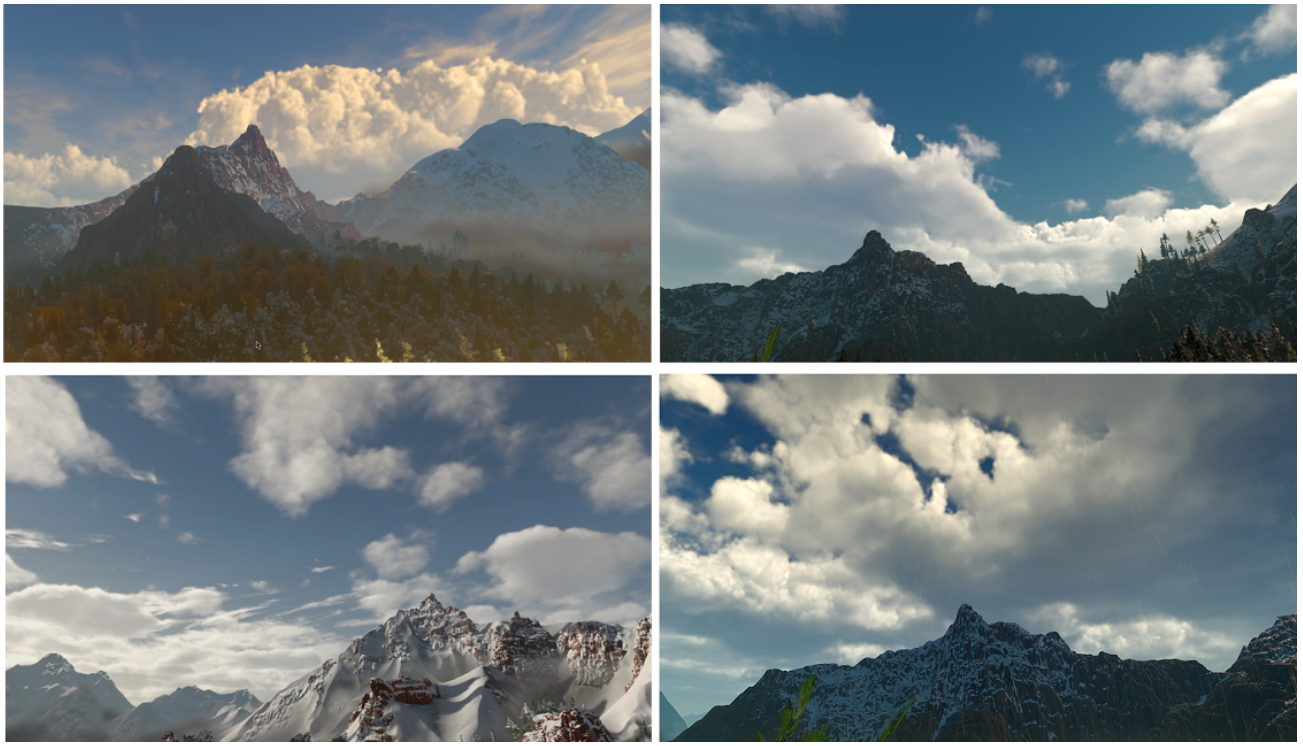
\includegraphics[width=13.83cm,height=9.1cm]{imagens/raymarched-clouds-schneider.png} 
    \caption{Raymarched Clouds obtained by Schneider et al.\protect\footnotemark}
    \label{fig:internet}
\end{figure}
\footnotetext{Source: Schneider et al.}

Ray Marching has found several practical applications in the gaming industry, particularly for rendering complex and dynamic scenes. In the Frostbite Engine [REFERENCIA], used in titles such as Battlefield V, Ray Marching is employed to render highly realistic volumetric clouds. This approach allows the engine to simulate depth, light scattering, and other atmospheric effects in real time, creating lifelike skies that respond dynamically to environmental lighting conditions. 

\footnotetext{Source: https://media.contentapi.ea.com/content/dam/eacom/frostbite/files/s2016-pbs-frostbite-sky-clouds-new.pdf}

\section{Scope and Objective}

In this document, we explore Ray Marching as implemented in GLSL and compare its strengths to traditional ray tracing methods. Our primary objective is to demonstrate Ray Marching's unique capabilities, particularly its use of SDFs, which allow for precise control over shapes and blending effects that are challenging to achieve with ray tracing.


We also explore the potential of Ray Marching for procedural rendering, showcasing its use in creating complex noise patterns and highly realistic volumetric effects, including cloud rendering. By examining these features, we aim to highlight Ray Marching’s versatility and its advantages in generating intricate, dynamic visuals for real-time applications.

\section{Methodology}

We take an iterative approach to explore the Ray Marching algorithm, showcasing its capacity to render smooth, noisy, and dynamic surfaces. Real-time 3D applications often rely on graphics APIs such as OpenGL, DirectX, or Vulkan for GPU programming. To simplify development and focus on Ray Marching itself, we use Shadertoy — a tool for running fragment shaders written in GLSL (OpenGL Shading Language) without the extensive setup. Fragment shaders are GPU programs that process each pixel on the screen, taking inputs such as the pixel position and canvas resolution.

\section{Text Structure}

O que cada capítulo fala. (pra depois)
\chapter{Ray Tracing vs Ray Marching}\label{chp:LABEL_CHP_2}

One of the goals of computer graphics is to synthesize images of virtual scenes simulating the behaviour of light. In order to determine the visible surfaces described in the environment and the respective color of each pixel displayed on the screen, two of the most widespread techniques are rasterization and ray tracing. Rasterization, widely used in real-time applications like video games, prioritizes speed and efficiency. In contrast, ray tracing, commonly employed in high-quality 3D animations, sacrifices speed for photorealistic accuracy by simulating the paths of individual light rays. Beyond these methods, ray marching offers a unique approach, particularly suited for rendering complex implicit surfaces and volumetric effects. In this chapter, we will focus on ray tracing and explore how it compares and contrasts with ray marching, shedding light on their respective strengths and applications.

\section{Traversing the Canvas}

A scene consists of a camera, 3D objects, and light sources placed in the environment. The goal when using ray tracing or ray marching is to generate a 2D render of the scene from the camera's point of view. We will need to traverse a 2D grid with the dimensions of our final image - the canvas. Then, given a camera point, we iterate over each position in the canvas, shooting a ray in its direction. This process is the basis of both ray marching and ray tracing.

% \begin{figure}[ht]
%     \centering
%     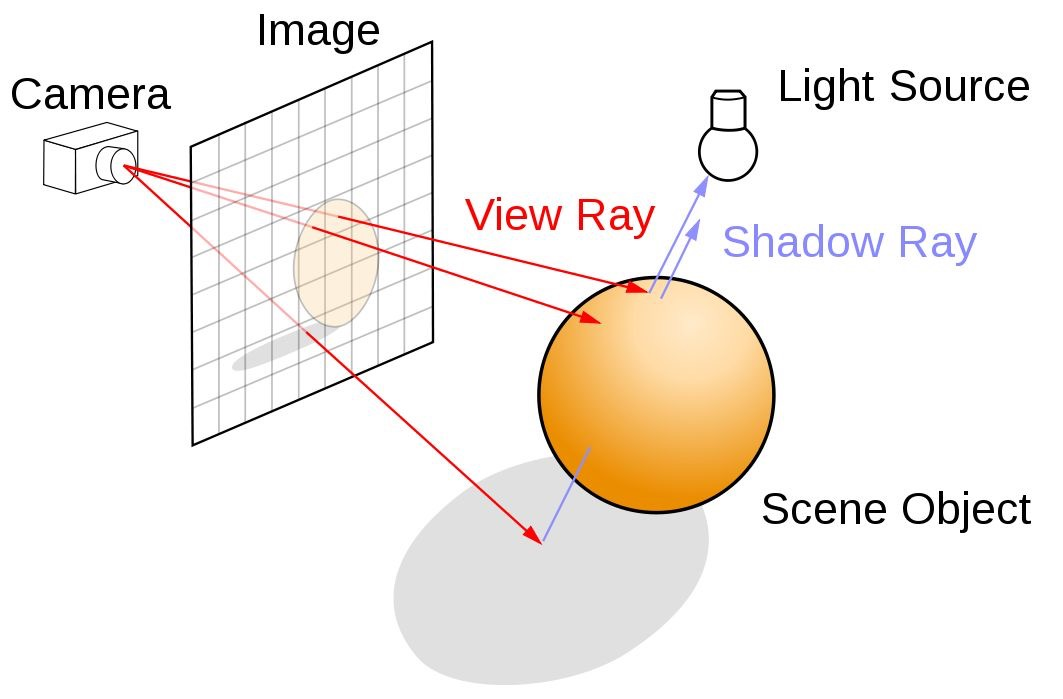
\includegraphics[width=10.64cm,height=7cm]{imagens/ray-trace.jpg} 
%     \caption{Ray Tracing Algorithm \protect\footnotemark}
%     \label{fig:internet}
% \end{figure}

For didactic purposes, we will ignore details such as the field of view, and we will assume that the distance between the canvas and the camera origin is always equal to 1, and that the canvas center will be positioned at $(0, 0, 0)$.

We are then able to establish the following definitions:

\begin{itemize}
    \item \textbf{CanvasResolution}: A 2D vector where each component represents the canvas' width and height.
    \item \textbf{uv} is a mapping of the canvas' coordinate system, offsetting the $(0, 0)$ coordinate to the canvas' center and ranging between -1 and 1. We later divide it by the resolution to fix the aspect ratio.
    \item \textbf{RayOrigin}: A 3D vector representing the viewer's position, initialized at $(0, 0, 1)$.
    \item \textbf{RayDirection}: A normalized 3D vector representing the ray shot from the origin towards the pixel's position.
    \item \textbf{Hit}: A data structure storing information about the ray's interaction with geometry, including hit position, surface normal, distance from the origin, and data for lighting calculations.
\end{itemize}

\footnotetext{Source: https://developer.nvidia.com/discover/ray-tracing}

The logic for traversing a 2D canvas and computing ray interactions with objects in the scene is outlined in \textbf{Algorithm 1 - Canvas Traversal}. This process applies to both ray tracing and ray marching, with the key difference being the implementation of the \texttt{TraceRay} function, used by ray tracing, which could be exchanged for \texttt{MarchRay}, used by ray marching.

\begin{algorithm}[H]
\caption{Canvas Traversal}
\begin{algorithmic}[1]
\Procedure{Render}{Canvas, Scene}
    \For{$y \gets 0$ to $CanvasResolution.y - 1$}
        \For{$x \gets 0$ to $CanvasResolution.x - 1$}
            \State $\mathbf{uv} \gets \left(\begin{bmatrix} x && y \end{bmatrix} - 0.5 * \text{CanvasResolution}\right) / CanvasResolution.y$
            \State $\mathbf{RayOrigin} \gets \begin{bmatrix} 0 && 0 && 1 \end{bmatrix}$
            \State $\mathbf{RayDirection} \gets \Call{normalize}{\begin{bmatrix} uv.x && uv.y && 0 \end{bmatrix} - \text{RayOrigin}}$
            \State $\mathbf{Hit} \gets \Call{TraceRay}{\mathbf{RayOrigin}, \mathbf{RayDirection}, \text{Scene}}$
            \If{$\text{Hit.isHit}$}
                \State $\mathbf{HitColor} \gets \Call{GetHitColor}{Hit, RayDirection, Scene}$
                \State $\Call{SetPixelColor}{x, y, \mathbf{HitColor}}$
            \Else
                \State $\Call{SetPixelColor}{x, y, \text{BACKGROUND\_COLOR}}$
            \EndIf
        \EndFor
    \EndFor
\EndProcedure
\end{algorithmic}
\end{algorithm}

The pseudocode explicitly uses nested loops to traverse the canvas. In the GLSL implementation that follows, the iteration logic is unnecessary because the fragment shader operates on a per-pixel basis. Each invocation of the shader corresponds to a single pixel on the canvas, and the GPU automatically handles the parallel execution of the shader for all pixels. The input \texttt{fragCoord} provides the current pixel's coordinates, \texttt{vec2} and \text{{vec3}} represent 2D and 3D vectors respectively, and GLSL functions handle vector operations like normalization and dot products. 


\begin{lstlisting}[language=GLSL, caption={Code 1: Canvas Traversal}, label={lst:CanvasTraversal} float=H]
void mainImage( out vec4 fragColor, in vec2 fragCoord )
{
    Scene scene = createScene();

    vec2 uv = (fragCoord - .5*iResolution.xy) / iResolution.y;
    vec3 color = vec3(0.);
    
    // Creating Ray
    vec3 rayOrigin = vec3(0., 0., 1.);
    vec3 rayDirection = normalize(vec3(uv.xy, 0.) - rayOrigin);
    Ray ray = Ray(rayOrigin, rayDirection);
    
    // Tracing Ray
    Hit hit = traceRay(ray, scene);
    
    if (hit.isHit) color = getHitColor(hit, ray, scene);
    
    // Output to screen
    fragColor = vec4(color,1.0);
}
\end{lstlisting}

\section{Tracing the Ray}

In ray tracing, once a ray is cast in the direction of a pixel on the canvas, it must traverse the scene to identify the closest object intersecting the ray. This requires a function capable of calculating the intersection between the ray and the geometric objects in the scene. The closest intersection point determines what will be rendered on the screen.


\begin{algorithm}[H]
\caption{TraceRay}
\begin{algorithmic}[1]
\Procedure{TraceRay}{RayOrigin, RayDirection, Scene}
    \State $ \mathbf{ClosestHit} \gets \text{RAYHIT\_INFINITY} $
    \ForEach {$\text{object} \in \text{Scene} $}
        \State $\mathbf{Hit} \gets \Call{RayObjectIntersection}{object, RayOrigin, RayDirection}$
        \If{$\text{Hit.distance} < \text{ClosestHit.distance}$}
            \State $\mathbf{ClosestHit} \gets \text{Hit}$
        \EndIf
    \EndFor
    \State \Return $\mathbf{ClosestHit}$
\EndProcedure
\end{algorithmic}
\end{algorithm}


In traditional computer graphics, most objects on a screen are represented as a collection of triangles. This allows any geometry tesselated into triangles to be described using ray-triangle intersection calculations. However, rendering smooth shapes requires an extremely fine mesh, leading to a high polygon count. This can create a significant performance bottleneck, especially in scenes containing thousands of objects, potentially resulting in millions of triangles.

In our example, we simplify the scene by using a single sphere. Since the mathematical formula for ray-sphere intersection is well-established\footnote{https://www.scratchapixel.com/lessons/3d-basic-rendering/minimal-ray-tracer-rendering-simple-shapes/ray-sphere-intersection.html}, it allows us to render a smooth and precise representation of the sphere without the need for tessellation.

The \texttt{GetHitColor} function currently returns only the object's albedo. To simulate realistic lighting behavior, additional calculations are required, which will be detailed in Chapter 3.

By rendering a scene with a black background, a large white sphere below the camera to simulate the ground, and a smaller red sphere above it, the image shown in Figure 3 is produced.

% \begin{figure}[ht]
%     \centering
%     \fbox{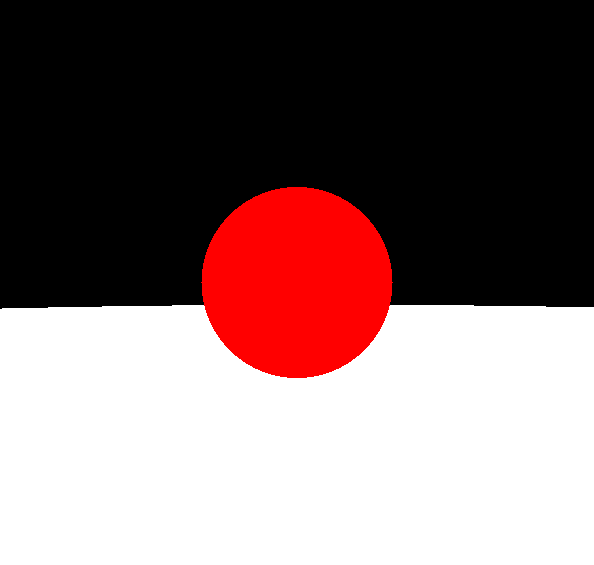
\includegraphics[width=7.64cm,height=7.64cm]{imagens/unlit-raytraced-sphere.png}}
%     \caption{Unlit Raytraced Sphere}
%     \label{fig:internet}
% \end{figure}


\section{Marching the Ray}

If the term `trace' implies a fast, swift motion, `march' is used to convey taking one step at a time. The ray marching algorithm uses the \texttt{MarchRay} function instead of \texttt{TraceRay}, so rather than calculating a direct intersection between the ray and the object, it resorts to iteratively marching through space, at each step sampling the distance to all objects in the scene, until one distance turns negative, or smaller than a specified threshold, which is considered a hit. The distance-sampling function is called SDF (Signed Distance Function), as it returns positive when outside the object, negative when inside. What is handy about SDF is that they are prone to various operations, chapter 3 will go though into some of them. 

Ray marching can be seen as a family of solvers, and there are variations of this process, on questions such as how to quantify the step size between samples. A traditional approach uses a fixed step size, in which the ray traverses space at constant steps. This has many applications, although when trying to render light in solids such as the sphere in Figure \ref{fig:internet}, the ray must be backtracked (Figure \ref{fig:spheretracing}), so as to obtain the exact collision point. Also, there is a chance of missing a collision altogether between samples (Figure \ref{fig:raymarch_fail}), especially when dealing with finely textured or detailed objects.

To prevent the march from ever skipping a surface between steps, instead of fixed, the next step size could be picked as the minimum distance between all samples to an object. The ray then acts as if it has a sensor, advising to march slower when surfaces are nearby. When a distance becomes smaller than a specified threshold, it`s considered a hit. This is observed in Figure \ref{fig:spheretracing}, at each step the circle's radius is a 2D representation of the minimum distance to a surface and thus the step size. In Algorithm \ref{alg:marchray} is the method described in code, in it the procedure \textsc{GetDistance}, at each step, calls within it the SDF of each object in scene, returning the minimum distance.

\begin{figure}[ht]
    \centering
    \fbox{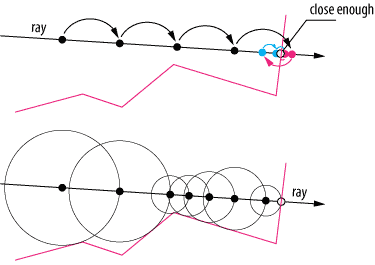
\includegraphics[width=7.64cm,height=5.40cm]{imagens/spheretracing.png}}
    \caption{Above, binary search maneuver to bypass fixed step limitations, below a display of Sphere Tracing}
    \label{fig:spheretracing}
\end{figure}

\begin{figure}[ht]
    \centering
    \fbox{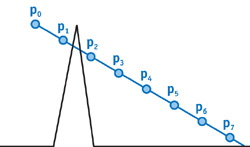
\includegraphics[width=7.64cm,height=4.49cm]{imagens/raymarch_fixed_fail.jpg}}
    \caption{A problematic case of fixed step, from section 8.3 of \cite{book:REF_BOOK_1}}
    \label{fig:raymarch_fail}
\end{figure}

\begin{figure}[ht]
    \centering
    \fbox{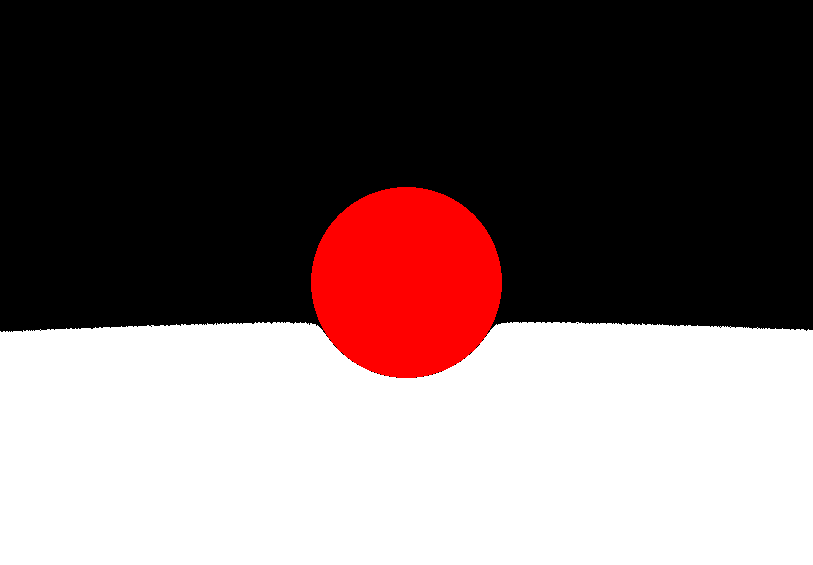
\includegraphics[width=7.64cm,height=5.30cm]{imagens/unlit-raymarched-sphere.png}}
    \caption{Unlit Raymarched Sphere}
    \label{fig:unlit_march_sphere}
\end{figure}

\begin{algorithm}[H]
\caption{MarchRay}
\label{alg:marchray}
\begin{algorithmic}[1]
\Procedure{MarchRay}{RayOrigin, RayDirection, Scene}
    \State $ \mathbf{MarchDistance} \gets \text{0} $
    \State $ \mathbf{Hit} \gets \text{NULL\_HIT} $
    \State $ \mathbf{IsHit} \gets \text{false} $
    \For {$step \gets 0$ to $\text{MAX\_MARCH\_STEPS} - 1$}
        \State $\mathbf{MarchPos} \gets  RayOrigin+ (MarchDistance * RayDirection) $
        \State $\mathbf{Hit} \gets \Call{GetDistance}{MarchPos, scene}$
        \If{$\text{Hit.distance} < \text{SURFACE\_DISTANCE}$}
            \State $ \mathbf{IsHit} \gets \text{true} $
            \State $ break $
        \EndIf
        \If{$\text{MarchDistance} > \text{MAX\_MARCH\_DISTANCE}$}
            \State $ break $
        \EndIf
    \EndFor
    \State \Return $\mathbf{Hit}$
\EndProcedure
\end{algorithmic}
\end{algorithm}

As to demonstrate a clear limitation of the method, Figure \ref{fig:unlit_march_sphere} was generated with a small 150 step limit. With close inspection, it`s possible to observe that the far away ground plane starts to disappear close to the edges of the ball. This is because the ray, when very close to objects, tends to march slow, and so it takes more steps to get through their borders, and in doing so hits the step limit and fails to reach what`s beyond, in the case of Figure \ref{fig:unlit_march_sphere} the ground. Fortunately, 150 steps is far from the optimal \texttt{MAX\_MARCH\_STEPS} number, a higher number can produce a featureless image with little additional computational costs, since most rays in the scene run into the ray distance limit sooner than 10 steps.

\section{When to march rather than trace}

At first glance, when comparing both methods, ray tracing comes off as the best, most optimal one. Ray marching is prone to visual features and might take a lot of marching steps to produce the best image, especially in crowded scenes. In the landscape of real-time computing, many companies also prioritize ray tracing over ray marching. Nowadays, most of the 3d modeling done in software like Blender and Zbrush is not based on primitives such as spheres and boxes, but rather on just polygons. As such, any traditionally modeled scene, with high poly counts, textures, reflection, refraction, shadows, is better off using ray tracing, especially considering the evolution of path tracing, and NVIDIA RTX's elegant optimizations, mixing rasterization in.

Now, it doesn`t mean ray marching has no competitive applications. Far from it, the flexibility of SDFs, and capability of diverse object combination and manipulation makes it particularly well-suited for rendering complex, mathematically defined shapes, such as fractals. Moreover, ray marching excels at rendering volumetric effects like clouds, fog, and smoke, which are inherently continuous and difficult to model with traditional polygonal geometry. By evaluating density functions at each step along a ray, ray marching can accurately simulate light scattering, absorption, and shadowing within these volumetric media.

Altough the demand for ray tracing specific hardware all but decreases, there is still a place for ray marching in real-time computing, even if it isn’t suited for rendering high-poly solid objects. It`s creative potential flourishes in communities like Shadertoy, where innovative ray-marched shaders showcase it's versatility. Beyond artistic applications, AAA games still leverage ray marching for realistic, dynamic effects like clouds characters fly through or smokes that bullets poke holes at. Additionally, in scientific fields, there are laboratories that apply ray marching on visualizations of all sorts, including 3D scalar fields, complex mathematical structures, such as Julia sets of quadratic functions and other quaternionic fractals. While its use cases may be more specialized, ray marching remains a powerful tool across both creative and technical domains, and hybrid solutions, using both marching and tracing, are widely adopted as to optimize the pros and cons of each method.

% Capítulo 3 (ou apêndice): Shading e Iluminação

% [O problema da visibilidade vs Shading]

% [Equação de Lambert, Phong e Ambiente]

% [Fog?]

% Casts de sombras

% Capítulo 4: SDFs e técnicas com ray marching

% Aprofundar a descrição da geometria através de SDFs
% Operações booleanas com SDFs: União, interseção, subtração
% Operações extras com SDFs: Smooth union, domain repetition

% Capítulo 5: Noise

% Explicações sobre white noise, value noise e FBM
% Exemplificação com Displacement

% Capítulo 6: Nuvem

% - Falta aprofundar um conhecimento pra concretizar o que escrever aqui
% - Beer's Law
% - Henyey-Greenstein?


% Capítulo 7: Observações, Resultados e Experimentos e Trabalhos Futuros

% is it possible to obtain a signed distance function giving a texture or a point cloud or a traditional 3D model?

% Is it possible to convert from SDF to a traditional 3D model?


% Capítulo 8: Conclusão

%\section{The Visibility Problem vs Shading}\label


%\section{}\label

%\section{}\label

% \section{Tables}\label{sec:LABEL_CHP_2_SEC_A}
% Reference: \url{http://en.wikibooks.org/wiki/LaTeX/Tables}

% \begin{table}[!h]
%   \centering
%   \begin{tabular}{ |l|l|l| }
%     \hline
%       Goalkeeper & Alan Smith & Paul Robinson \\
%     \hline
%       Lucus Radebe &  Mark Viduka & Michael Duberry \\
%     \hline
%       Eirik Bakke & Jamie McMaster & Jody Morris \\
%     \hline
%   \end{tabular}
%   \caption{This table shows some data}
%   \label{tab:LABEL_TAB_1}
% \end{table}

% \section{Images}\label{sec:LABEL_CHP_2_SEC_B}
% Reference: \url{http://en.wikibooks.org/wiki/LaTeX/Importing_Graphics}

\begin{figure}[h]
  \centering
  
\includegraphics[width=0.3\textwidth]{imagens/chick.png}
  \caption{Chick}
  \label{fig:LABEL_FIG_1}
\end{figure}

% \section{Equations}\label{sec:LABEL_CHP_2_SEC_C}
% Reference: \url{http://en.wikibooks.org/wiki/LaTeX/Mathematics}

% Also: \url{http://en.wikibooks.org/wiki/LaTeX/Advanced_Mathematics}

% \begin{equation}
%   (x + y)^2 = x^2 + 2xy + y^2
%   \label{eq:LABEL_EQ_1}
% \end{equation}

% \section{Listings}\label{sec:LABEL_CHP_2_SEC_D}
% Reference: \url{http://en.wikibooks.org/wiki/LaTeX/Source_Code_Listings}

% \codec{C}{alg:LABEL_CODE_1}{codigos/codigo-c.txt}

% \codejava{Java}{alg:LABEL_CODE_2}{codigos/codigo-java.txt}

% \section{References}\label{sec:LABEL_CHP_2_SEC_E}
% \begin{itemize}
%   \item Referencing \refchapter{chp:LABEL_CHP_1}
%   \item Referencing \refsection{sec:LABEL_CHP_1_SEC_A}
%   \item Referencing \refsection{sec:LABEL_CHP_1_SEC_C}
%   \item Referencing \reftable{tab:LABEL_TAB_1}
%   \item Referencing \reffigure{fig:LABEL_FIG_1}
%   \item Referencing \refequation{eq:LABEL_EQ_1}
%   \item Referencing \reflisting{alg:LABEL_CODE_1}
%   \item Article \cite{art:REF_ART_1}
% %   \item Referencing \refappendix{chp:LABEL_APP_1}
% \end{itemize}
\chapter{Signed Distance Functions Techniques}\label{chp:LABEL_CHP_2}

A \textit{Signed Distance Function} (SDF) provides a way to describe geometric forms in a continuous manner by associating each point in space with its \textit{signed distance} to a surface. The function returns positive value when the point is outside the shape and a negative value when the point is inside the shape. This framework is highly flexible, allowing the representation of shapes in 2D, 3D, and even N-dimensional spaces, since the Euclidean distance is not restricted to a particular number of dimensions.  

A defining feature of Ray Marching is its use of signed distance functions to describe geometry, rather than traditional vertices, edges, and faces. This approach is precisely what makes Ray Marching a powerful technique, capable of rendering of smooth surfaces, shapes distorted by procedural noise, repetitive patterns, fractals, and dynamic shapes that evolve over time.
    
This chapter further describes signed distance functions for basic shapes and explores techniques for constructing complex shapes by combining and manipulating the fields to achieve the desired scene composition.

% https://www.shadertoy.com/view/lslXD8

\section{Basic Shapes}


The general form of an SDF function includes:  

\begin{itemize}
    \item $\mathbf{p}$, the \textbf{query point}, for which the distance from the shape positioned at the origin is computed.
    \item Shape-specific parameters, such as the \textbf{radius} for circles and spheres, or additional properties like \textbf{width, height, or orientation} for more complex geometries.
\end{itemize}

\subsection{Circles and Spheres}

For a circle centered at the origin in $ \mathbb{R}^ 2 $ with radius $r$, the SDF is given by:

$$\text{CircleSDF}(\mathbf{p}) = \|\mathbf{p}\| - r$$

A sphere in three-dimensional space follows the same principle. If the sphere is centered at the origin with radius $r$, the SDF becomes:

$$\text{SphereSDF}(\mathbf{p}) = \|\mathbf{p}\| - r$$


where $\mathbf{p}$ in $\mathbb{R}^3 $ is now a point in three-dimensional space.

The only difference between the circle and the sphere is the dimension of the query point $\mathbf{p}$. In the case of a circle, $\mathbf{p}$ is a two-dimensional vector, whereas for a sphere, $\mathbf{p}$ is a three-dimensional vector. The formula remains structurally identical because both objects are defined by a center and a radius in their respective spaces.

\begin{lstlisting}[language=GLSL, caption={Code 2: Circle and Sphere SDFs}, label={lst:CircleAndSphere} float=H]
float circleDistance(vec2 point, float radius){
    return length(point) - radius;
}

float sphereDistance(vec3 point, float radius){
    return length(point) - radius;
}
\end{lstlisting}

Since an SDF returns a positive distance when a point is outside the primitive and a negative distance when inside, this information can be used to assign different colors to a 2D shape rendered on the canvas.

\begin{lstlisting}[language=GLSL, caption={Code 3: Rendering Circles}, label={lst:ColoringCircle} float=H]
vec3 plainColor (in float d){
     return vec3(1.0) - sign(d)*vec3(0.4);
}

void mainImage( out vec4 fragColor, in vec2 fragCoord )
{
    vec2 uv = (2.*fragCoord.xy-iResolution.xy)/min(iResolution.x, iResolution.y);

    float d = circleDistance(uv, 0.5);

    vec3 col = plainColor(d);
    fragColor = vec4(col,1.0);
}
\end{lstlisting}

\begin{figure}
\centering
\begin{minipage}{.5\textwidth}
  \centering
  
\includegraphics[width=.8\linewidth]{imagens/circle-plainColor.png}
  \captionof{figure}{Plain Colored Circle}
  \label{fig:plainColoredCircle}
\end{minipage}%
\begin{minipage}{.5\textwidth}
  \centering
  
\includegraphics[width=.8\linewidth]{imagens/circle-customColor.png}
  \captionof{figure}{Custom Colored Circle}
  \label{fig:customColoredCircle}
\end{minipage}
\end{figure}

In Figure \ref{fig:plainColoredCircle}, it is possible to see the color outside the circle being rendered in a darker shade than inside the circle. The implementation for such render can be seen in Code 3. For the following shapes, we will use a custom coloring function that adds isolines and highlights the border, as shown in Figure \ref{fig:customColoredCircle}. This technique allows the visualization of 2D SDFs in the distance space.

3D Signed Distance Functions (SDFs) define the shapes of objects within a scene in the Ray Marching pipeline. For instance, the distance function of a sphere can represent the scene's minimum distance in the \texttt{createScene} function (see Code 1). Rays are marched accordingly, and collision information is passed to the \texttt{getHitColor} function. As previously discussed, this process closely resembles both Ray Marching and Ray Tracing techniques, including the lighting calculations used to shade the hit point. The following examples in this chapter illustrate 3D SDFs rendered with Lambertian diffuse shading and Phong specular reflection.

\begin{figure}[ht]
    \centering
  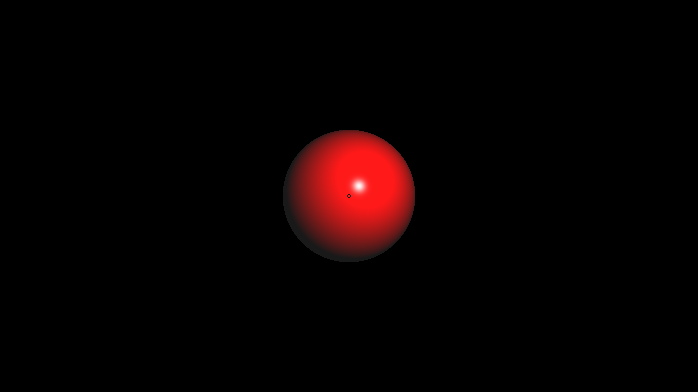
\includegraphics[width=.6\linewidth]{imagens/sdf-sphere.png}
  \captionof{figure}{Raymarched Sphere SDF Visualization}
  \label{fig:sdf-sphere}
\end{figure}

Since lighting models are outside the scope of this essay, readers may refer to Real-Time Rendering, 4th Edition by Akenine-Möller et al. for further details on shading techniques \cite{akenine-moller2018realtimerendering}.

\subsection{Rectangles and Boxes}

% \begin{figure}[ht]
%     \centering
%   
\includegraphics[width=.6\linewidth]{imagens/rectangle-customColor.png}
%   \captionof{figure}{Rectangle SDF Visualization}
%   \label{fig:customColoredRectangle}
% \end{figure}

Similar to the 2D circle, the signed distance function (SDF) of a 2D box, or rectangle, can be generalized to higher dimensions.

\begin{lstlisting}[language=GLSL, caption={Code 4: Rectangle and Box SDF}, label={lst:RectangleAndBox} float=H]
float rectangleDistance( in vec2 p, in vec2 b ){
    vec2 d = abs(p)-b;
    return length(max(d,0.0)) + min(max(d.x,d.y),0.0);
}

float boxDistance( in vec3 p, in vec3 b ){
    vec3 d = abs(p)-b;
    return length(max(d,0.0)) + min(max(d.x,d.y,d.z),0.0);
}
\end{lstlisting}

The rectangle SDF is defined at the origin $\mathbf{[0,0]}$, and due to the rectangle's symmetry, it is often more convenient to work within the first cartesian quadrant. To achieve this, $\mathbf{b}$ (half each box`s side) is subtracted from $\mathbf{abs(p)}$, yielding a point $\mathbf{d}$. As illustrated in Figure \ref{fig:square_sdf}:

\begin{itemize}
    \item If only $\mathbf{d.x<0}$, it indicates that $\mathbf{p}$ is above the rectangle, in section 1, and the shortest distance is straight down.
    \item If only $\mathbf{d.y<0}$, it means that $\mathbf{p}$ is next to the rectangle, in section 3, so the shortest distance is straight left.
    \item If both $\mathbf{d.x}<0$ and $\mathbf{d.y<0}$, the point is inside the rectangle, in section 4, thus the shortest distance is the closest of the two sides.
    \item Finally, if neither component is negative, the point lies diagonally outside the rectangle, in section 2, so the distance to the corner is the shortest.
\end{itemize}

\begin{figure}[ht]
    \centering
    \fbox{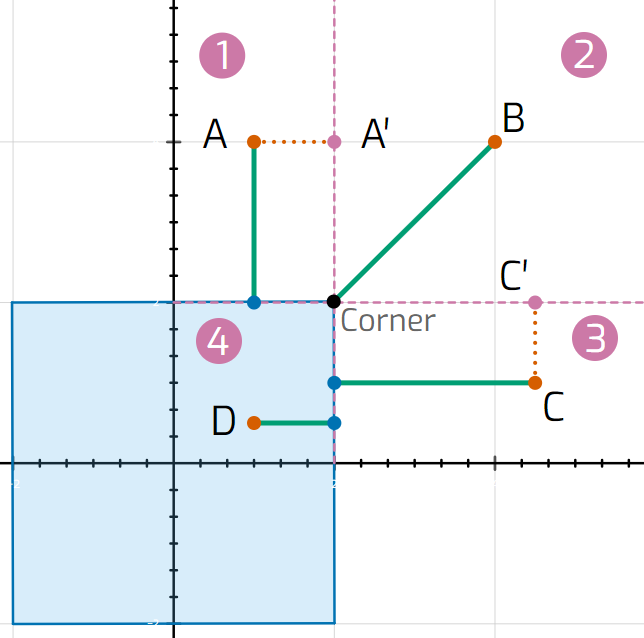
\includegraphics[width=7.5cm,height=7.43cm]{imagens/square_sdf.png}}
    \caption{Graphic of Rectangle SDF calculation}
    \label{fig:square_sdf}
\end{figure}

It can be seen that when both $\mathbf{d.x}$ and $\mathbf{d.y}$ are limited to zero, which visually means snapping all points to section 2, the distance to the corner encases the results, although not entirely. If in section 4, inside the rectangle, $\mathbf{length(max(d,0.0))}$ is always 0. In such cases, the SDF should return the negative distance to the nearest edge of the rectangle, adding the expression $\mathbf{min(max(d.x,d.y),0.0)}$. The min() function ensures non-zero distances are only possible in section 4. With that, all sections are considered.

This process can be generalized to higher dimensions in a similar fashion. As such, the 3D box SDF can be derived by extending the approach to $\mathbb{R}^3 $, where p and b are now three-dimensional vectors.


\begin{figure}[ht]
    \centering
  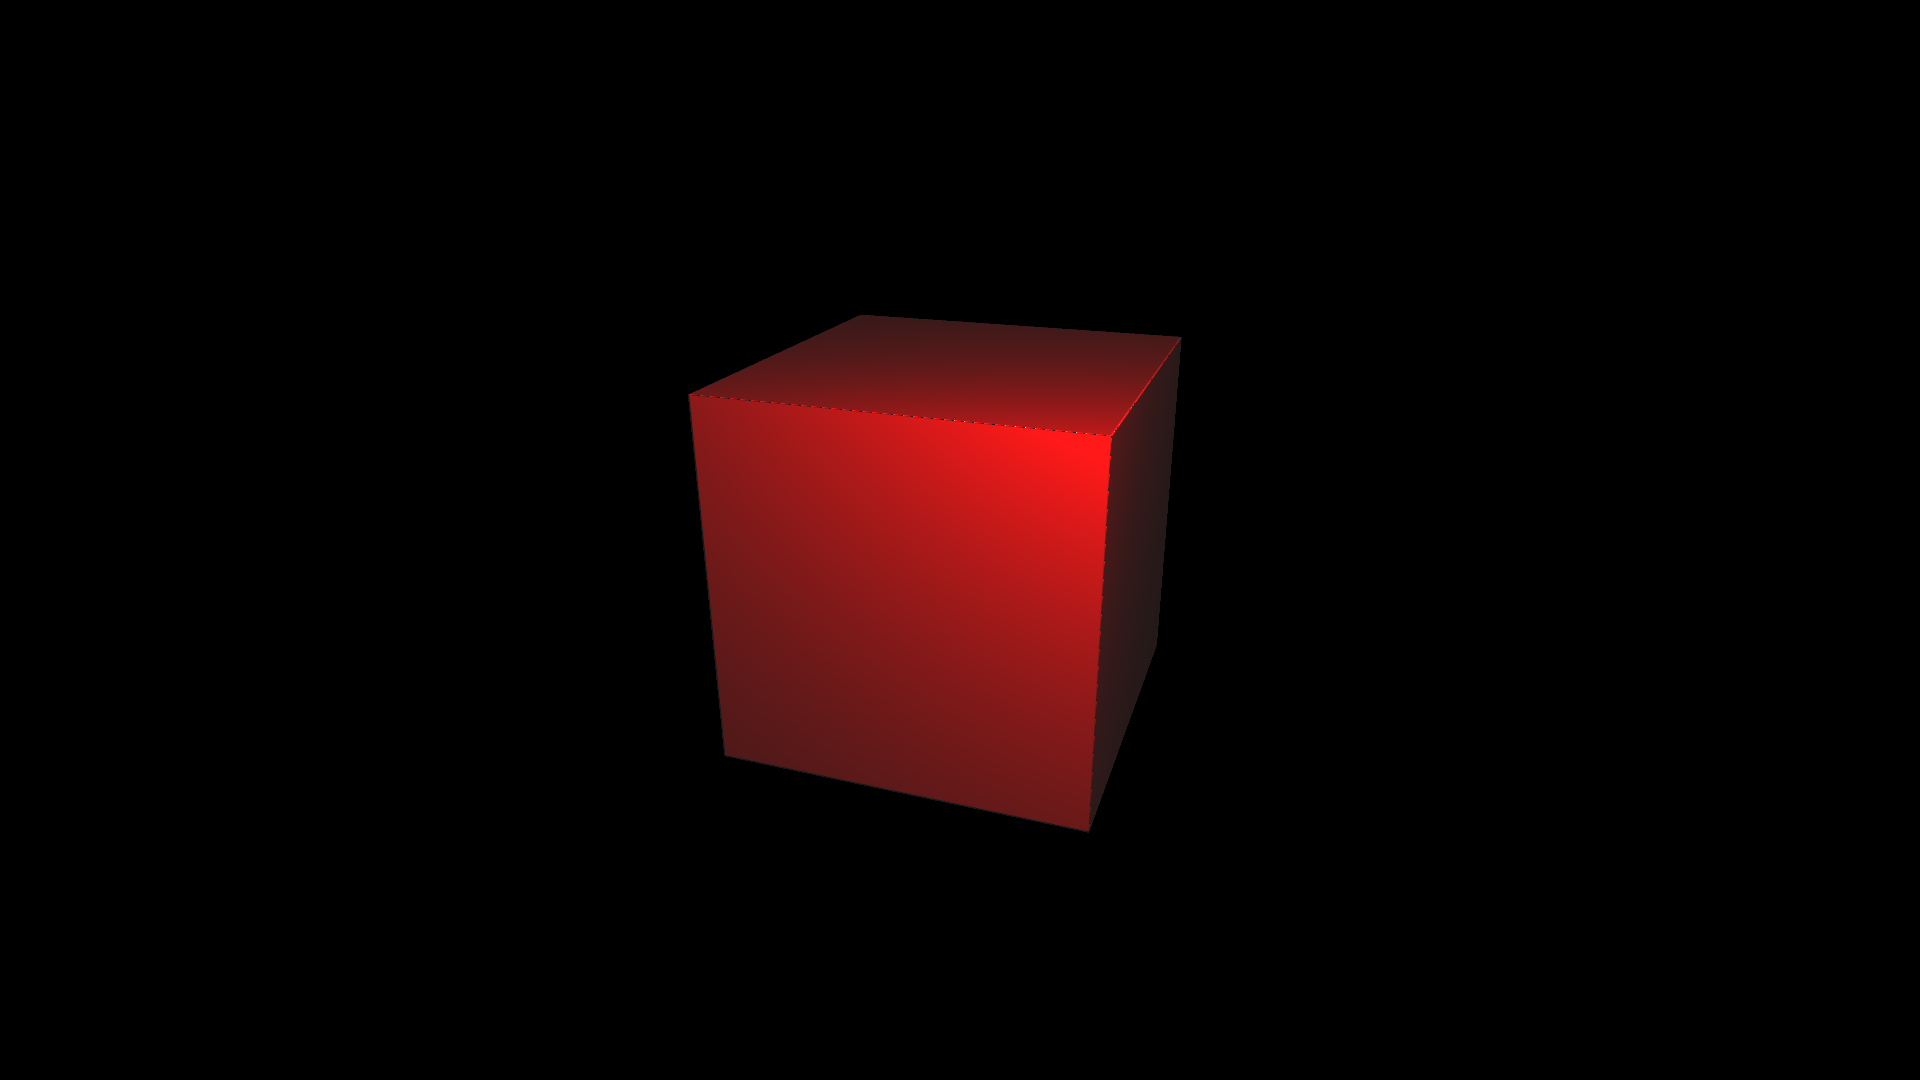
\includegraphics[width=.6\linewidth]{imagens/sdf-cube.png}
  \captionof{figure}{3D Cube SDF Visualization}
  \label{fig:sdf-cube}
\end{figure}


If expanded to $\mathbb{R}^4 $, the SDF can help visualize forms such as the tesseract, the 4D hypercube, by fixing and scrolling through one of the four axes.

\section{Basic Transformations}

All primitive described in the previous section were centered at the origin. In order to perform a transformation such as scaling, rotation or translation, it is possible to apply the transformation at the query point $\mathbf{p}$.

%BOTAR EXEMPLO DE CODIGO FACIL
%vec3 opTransformRotate( in vec3 p, in transform t, in sdf3d primitive ){
%    return primitive( invert(t)*p );
%}
%float opScale( in vec3 p, in float s, in sdf3d primitive ){
%    return primitive(p/s)*s;
%}

%UM PARAGRAFO PRA EXPLICAR RAPIDINHO

\section{Operations}

While being able to display a variety of primitives is great, both ray tracing and ray marching have such capabilities. As time goes by, what is required of modern computer graphics becomes much more than that, and in search of building more complex forms is where both methods part ways. While ray tracing depends on high polygon-count models, almost never using other types of primitives, ray marching finds more success with a variety of solutions, one such being the use of various combinations between primitives and operations as building blocks.
This section describes some of the main SDF operations used in modeling based on basic primitives. Having primitives centered at the origin also facilitates many of the operations.

\subsection{Union, Intersection and Subtraction}

Operations between objects are some of the most elegant features of SDFs, and the most basic ones are the combinations: Union, Intersection and Subtraction. These three have very simple definitions and are great ways to introduce SDF operations. They take as input the SDF resulting distance of two primitive SDFs.


\begin{lstlisting}[language=GLSL, caption={Code 5: SDF Union, Intersection and Subtraction}, label={lst:UnionIntersectionSubtraction} float=H]
float unionOperation( float d1, float d2 )
{
    return min(d1,d2);
}
float intersectionOperation( float d1, float d2 )
{
    return max(d1,d2);
}
float subtractionOperation( float d1, float d2 )
{
    return max(-d1,d2);
}
\end{lstlisting}

From the perspective of a 3D raymarched vision, given $\mathbf{d1}$ and $\mathbf{d2}$, SDF distances from objects 1 and 2:

\begin{itemize}
    \item Taking the minimum between $\mathbf{d1}$ and $\mathbf{d2}$ is like seeing only the closest surface from both objects to camera, which is already the case for solids seen from the outside.
    \item Taking the maximum between $\mathbf{d1}$ and $\mathbf{d2}$ means that nothing outside the intersection of both objects is seen, since the ray march will only consider a hit if both SDF results are below the hit threshold.
    \item Taking the maximum between $\mathbf{-d1}$ and $\mathbf{d2}$ is like intersecting with the inverse of d1, which means that all $\mathbf{R}^3 $ except object1. This results in the subtraction of objects 1 from 2.
\end{itemize}


\begin{figure}[h!]
    \centering

    % Row 1
    \begin{minipage}{0.3\textwidth}
        \centering
        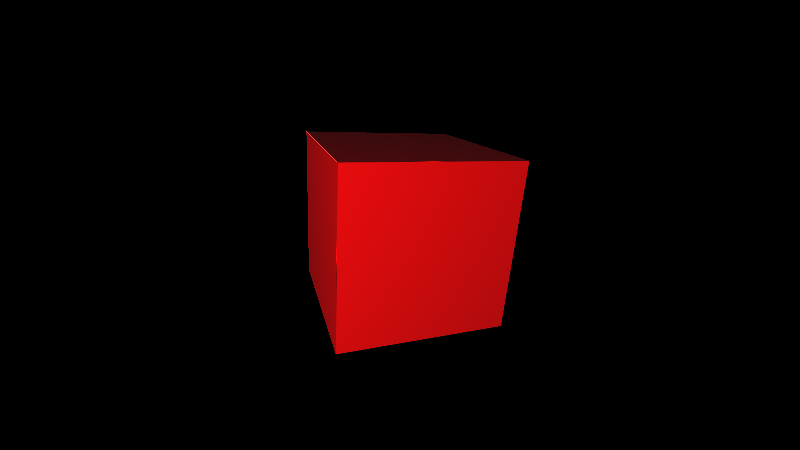
\includegraphics[width=\linewidth]{imagens/sdf-operations/cube.png}\\
        Cube
    \end{minipage}%
    \hfill
    \begin{minipage}{0.3\textwidth}
        \centering
        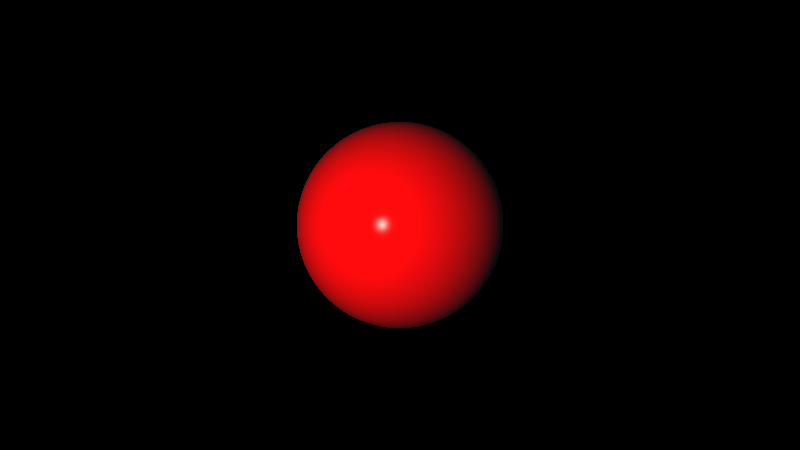
\includegraphics[width=\linewidth]{imagens/sdf-operations/sphere.png}\\
        Sphere
    \end{minipage}%
    \hfill
    \begin{minipage}{0.3\textwidth}
        \centering
        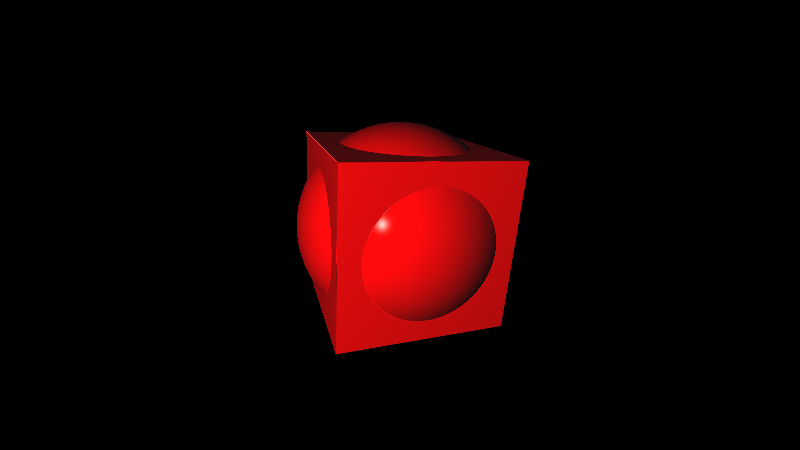
\includegraphics[width=\linewidth]{imagens/sdf-operations/union.png}\\
        Union
    \end{minipage}

    \vspace{1em} % space between rows

    % Row 2
    \begin{minipage}{0.3\textwidth}
        \centering
        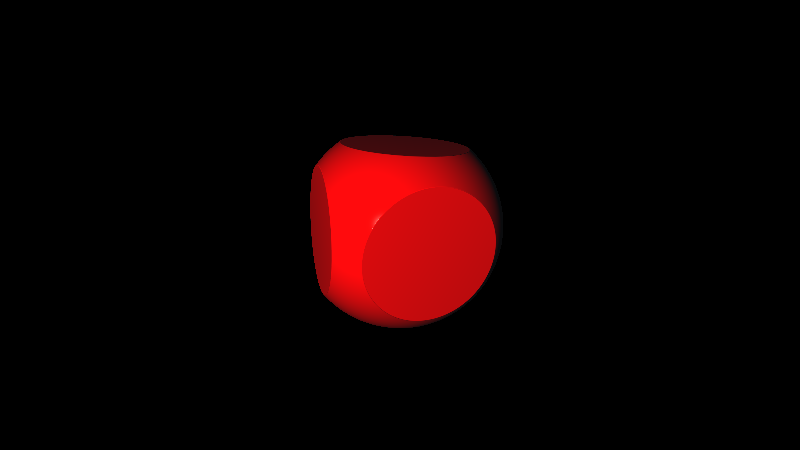
\includegraphics[width=\linewidth]{imagens/sdf-operations/intersection.png}\\
        Intersection
    \end{minipage}%
    \hfill
    \begin{minipage}{0.3\textwidth}
        \centering
        
\includegraphics[width=\linewidth]{imagens/sdf-operations/subtraction1.png}\\
        Subtraction 1
    \end{minipage}%
    \hfill
    \begin{minipage}{0.3\textwidth}
        \centering
        
\includegraphics[width=\linewidth]{imagens/sdf-operations/subtraction2.png}\\
        Subtraction 2
    \end{minipage}

    \caption{Raymarched Constructive Solid Geometry Operations with Cube and Sphere SDFs.}
    \label{fig:sdf_operations}
\end{figure}

\subsection{Smooth Union, Intersection and Subtraction}

A more complicated, yet visually appealing way to display the basic boolean operations is through the use of Smooth Minimum and Maximum. As the name implies, instead of binary hard edge transitions between the primitives, it offers a smooth blend. Figures \ref{fig:sunion}, \ref{fig:sinter} and \ref{fig:ssub} combine the same box and circle with each smooth variant of the basic operations.
This blending can be achieved through multiple types of functions, such as quadratic, cubic, exponential, sigmoid, each having it`s pros and cons.

\begin{figure}
\centering
\begin{minipage}{.5\textwidth}
  \centering
  
\includegraphics[width=.8\linewidth]{imagens/smoothUnion.png}
  \captionof{figure}{Smooth Union}
  \label{fig:sunion}
\end{minipage}%
\begin{minipage}{.5\textwidth}
  \centering
  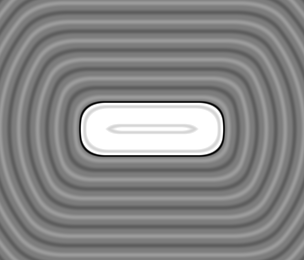
\includegraphics[width=.8\linewidth]{imagens/smoothIntersection.png}
  \captionof{figure}{Smooth Intersection}
  \label{fig:sinter}
\end{minipage}
\end{figure}
\begin{figure}
\centering
\begin{minipage}{.5\textwidth}
  \centering
  
\includegraphics[width=.8\linewidth]{imagens/smoothSubtraction.png}
  \captionof{figure}{Smooth Subtraction}
  \label{fig:ssub}
\end{minipage}%
\begin{minipage}{.5\textwidth}
  \centering
  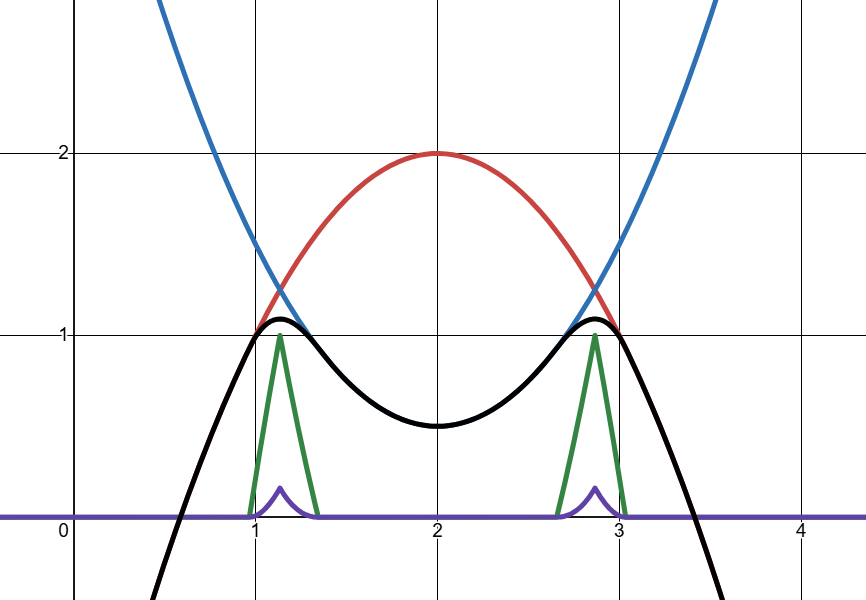
\includegraphics[width=.8\linewidth]{imagens/desmos_smin.png}
  \captionof{figure}{Smooth Minimum Representation}
  \label{fig:smin}
\end{minipage}
\end{figure}

Because it is fast and does not overestimate distances, the quadratic polynomial is less prone to visual artifacts and is the most widely used version for ray marching, thus being the one this section focuses on. Similarly to the regular min function, smin (smooth minimum) takes as input $\mathbf{a}$ and $\mathbf{b}$, which could be distances, or points in space, plus the threshold $\mathbf{k}$. The blending starts where the distance between $\mathbf{a}$ and $\mathbf{b}$ is smaller than $\mathbf{k}$.

Figure \ref{fig:smin} will help navigate the explanation ahead, $\mathbf{a\ =\ -\left(2-x\right)^{2}+2}$ is in red and $\mathbf{b\ =\ \left(2-x\right)^{2}\ +.5}$ in blue. To find smin, all polynomial methods start by finding the $\mathbf{h()}$ function, which is 0 by default, and ramps up to 1, starting at $\mathbf{|a - b|=k}$ and peaking at $\mathbf{|a - b|=0}$:

\begin{equation}
    h = \frac{\max(k - |a - b|, 0.0)}{k}
    \label{eq:example_equation}
\end{equation}

Since $\mathbf{k}$ is the distance in which the shapes start to combine, $\mathbf{h()}$ helps delimitate exactly that, as represented in green, Figure \ref{fig:smin}. Next, there needs to be a $\mathbf{c}$ such that $\mathbf{min(a,b)-c}$ produces the smoothed curve. This is no random requirement, but a simplified structure of what is the DD (Direct Difference) family of smin solutions. For polynomials, a simple solution for $\mathbf{c}$ is as follows, with $\mathbf{n>1.5}$ already producing great results:

\begin{equation}
    c\ =\frac{h^{n}k}{2n}
    \label{eq:example_equation}
\end{equation}

Between all values of $\mathbf{n}$, the quadratic version ($\mathbf{n=2}$) produces the gentler of curves, and is prioritized over the others. To better visualize what $\mathbf{c}$ means, Figure \ref{fig:sunion} represents $\mathbf{c}$ in purple. Squaring $\mathbf{h}$ makes c ease into 1, instead of following a straight ramp. Multiplying by $\mathbf{k}$ compensates any variation, as the peak of $\mathbf{h}$ decreases as $\mathbf{k}$ increases. Lastly, the divisor helps position the peak to the right place.
To achieve smooth maximum, all that is needed is $\mathbf{max(a,b)+c}$.

\begin{figure}[h!]
    \centering

    % Row 1
    \begin{minipage}{0.3\textwidth}
        \centering
        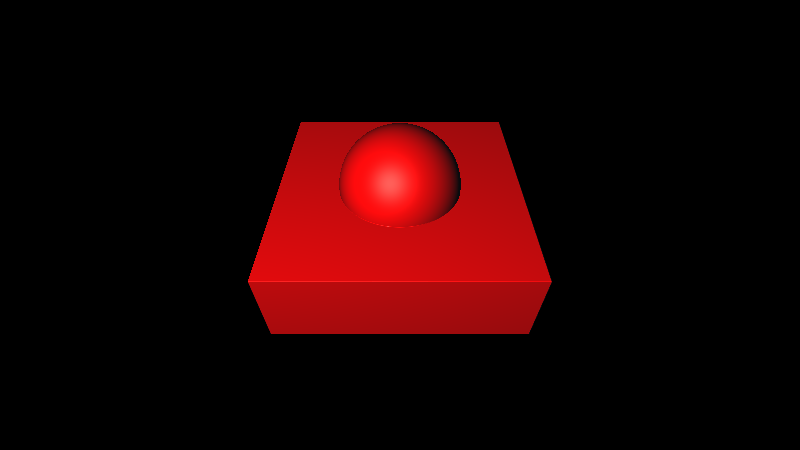
\includegraphics[width=\linewidth]{imagens/smooth-sdf-operations/add-unsmooth.png}\\
        Addition
    \end{minipage}%
    \hfill
    \begin{minipage}{0.3\textwidth}
        \centering
        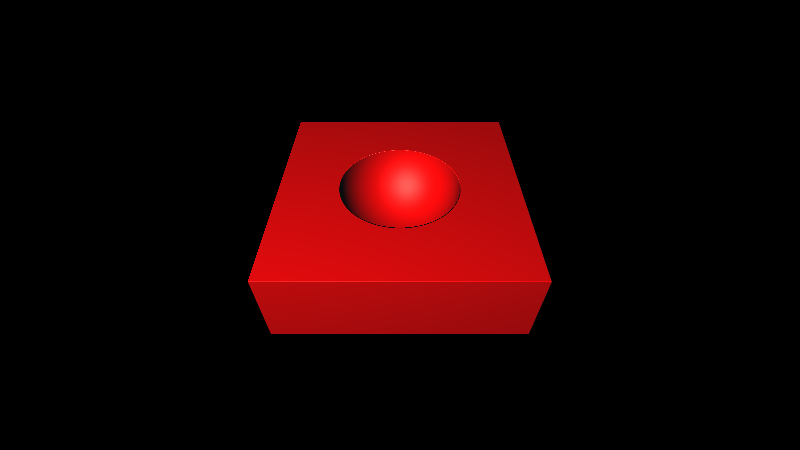
\includegraphics[width=\linewidth]{imagens/smooth-sdf-operations/subtraction-unsmooth.png}\\
        Subtraction
    \end{minipage}%
    \hfill
    \begin{minipage}{0.3\textwidth}
        \centering
        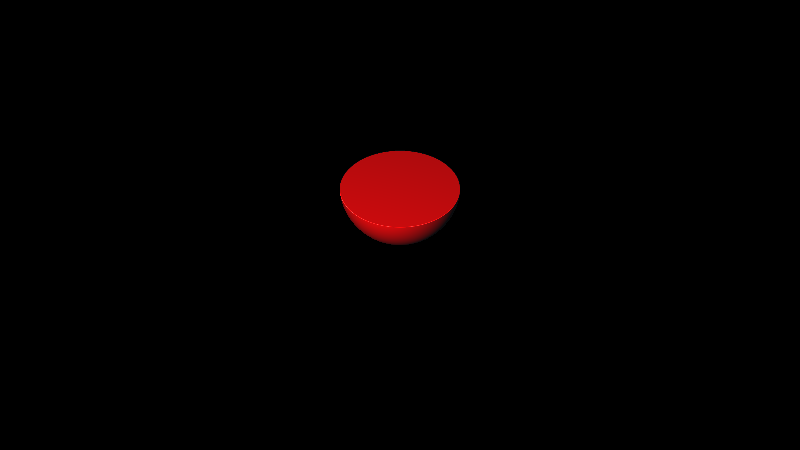
\includegraphics[width=\linewidth]{imagens/smooth-sdf-operations/intersection-unsmooth.png}\\
        Intersection
    \end{minipage}

    \vspace{1em} % space between rows

    % Row 2
    \begin{minipage}{0.3\textwidth}
        \centering
        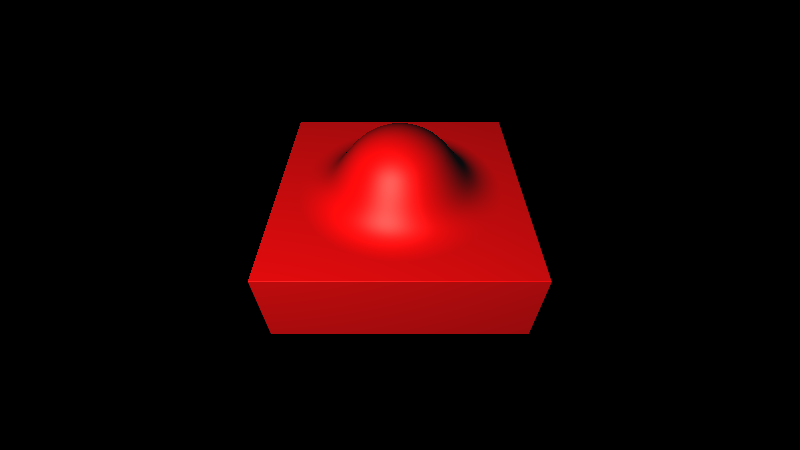
\includegraphics[width=\linewidth]{imagens/smooth-sdf-operations/add-smooth.png}\\
        Smooth Addition
    \end{minipage}%
    \hfill
    \begin{minipage}{0.3\textwidth}
        \centering
        
\includegraphics[width=\linewidth]{imagens/smooth-sdf-operations/subtraction-smooth.png}\\
        Smooth Subtraction
    \end{minipage}%
    \hfill
    \begin{minipage}{0.3\textwidth}
        \centering
        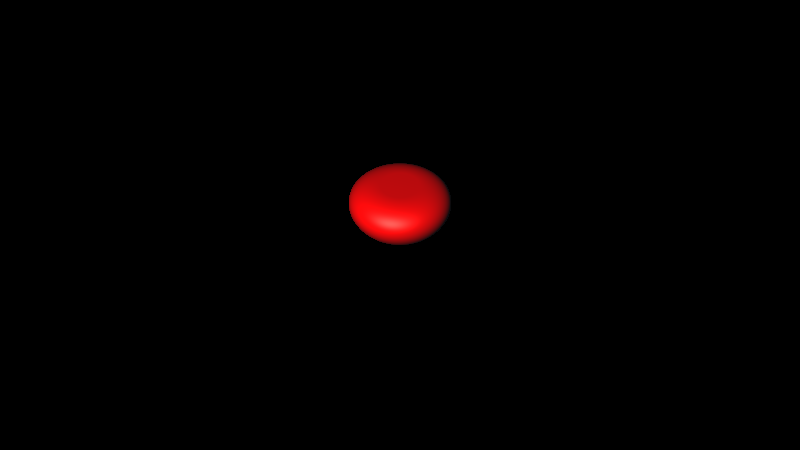
\includegraphics[width=\linewidth]{imagens/smooth-sdf-operations/intersection-smooth.png}\\
        Smooth Intersection
    \end{minipage}

    \caption{Raymarched Smooth Operations with Cube and Sphere SDFs.}
    \label{fig:smooth_sdf_operations}
\end{figure}

\subsection{Domain Repetition}

Since SDFs are expressed as mathematical functions, they can be transformed to repeat periodically across space. This technique, known as domain repetition, allows for the creation of infinite, repeating patterns in a scene while also optimizing performance by avoiding the need for multiple individual primitives.

There are many variations of this technique, as any domain parametrization can be made repeating, but the core idea is to use mathematical operations that will result in the desired scene. 

This can be achieved through the natural repetitive pattern of trigonometric functions such as $sin(x)$ and $cos(x)$, however, bending the domain with these functions will compromise the accurate Euclidean distances of the space the SDFs relies on, and this might generate unwished features. Functions such as $round(x)$ or $mod(x)$ (modulus operator) are more commonly used instead.

\begin{figure}[h!]
    \centering

    % Row 1
    \begin{minipage}{0.45\textwidth}
        \centering
        
\includegraphics[width=\linewidth]{imagens/domainRepetition-circle.png}\\
        circleDistance(uv, 0.1)
    \end{minipage}%
    \hfill
    \begin{minipage}{0.45\textwidth}
        \centering
        
\includegraphics[width=\linewidth]{imagens/domainRepetition-sine.png}\\
        circleDistance(sin(uv * 5.)*0.2, 0.1)
    \end{minipage}

    \vspace{1em} % space between rows

    % Row 2
    \begin{minipage}{0.45\textwidth}
        \centering
        
\includegraphics[width=\linewidth]{imagens/domainRepetition-round.png}\\
        circleDistance(uv - round(uv), 0.1)
    \end{minipage}%
    \hfill
    \begin{minipage}{0.45\textwidth}
        \centering
        
\includegraphics[width=\linewidth]{imagens/domainRepetition-mod.png}\\
        circleDistance(mod(uv, 1.)-0.5, 0.1)
    \end{minipage}

    \caption{Examples of Domain Repetition techniques.}
    \label{fig:domainRepetition}
\end{figure}

Given that \textbf{uv} represents the query point in the domain, with the zero vector centered on the canvas, Figure \ref{fig:domainRepetition} illustrates the output of the custom coloring function applied to its respective transformation. Naturally, this can also be used in 3D: Given that $\mathbf{p}$ represents the query point in the domain, the repeated domain can be represented as 
$\mathbf{p} - \textit{gap} \cdot \mathrm{round}\!\left( \frac{\mathbf{p}}{\textit{gap}} \right)$,
where \textit{gap} is the size of the repeated domain box. Figure~\ref{fig:sdf-3d-domainRepetition} 
shows an example of repeated spheres in a repeated domain.

\begin{figure}[ht]
    \centering
  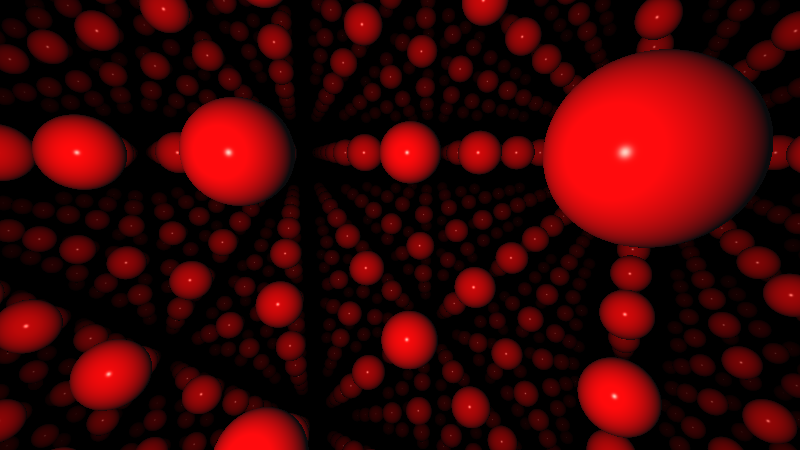
\includegraphics[width=.6\linewidth]{imagens/domain-repetition.png}
  \captionof{figure}{sphereDistance(p - 6.5*round(p/6.5), 1.0)}
  \label{fig:sdf-3d-domainRepetition}
\end{figure}

\subsection{Displacement}

Displacement is a technique used to adjust the geometry to simulate bumps or irregularities, adding fine detail to the surface. This is often done by perturbing the distance field using patterns that look random, such as static or grain, which can be generated with mathematical formulas (procedural noise) or taken from images (noise textures).

\begin{lstlisting}[language=GLSL, caption={Code 6: SDF Displacement}, label={lst:Displacement} float=H]
float displacementOperation( in sdf3d sdfShape, in vec3 p )
{
    float d1 = sdfShape(p);
    float d2 = displacement(p);
    return d1+d2;
}
\end{lstlisting}

Although noisy functions are commonly used for displacement, any function can be applied to distort the distance field. This flexibility enables the creation of non-Euclidean effects, such as bending or twisting space. However, this comes with a caveat: the sum of an SDF and an arbitrary function is not necessarily an SDF.

A key property of 2D and 3D Signed Distance Functions is that their gradient has length $1.0$ everywhere in the space. Since SDFs measure distances, the rate of change of distance must be equal to 1.0. When two SDFs are added, this property is violated — the gradient no longer has unit length, effectively "bending" space. This can cause the raymarcher to underestimate or overestimate the true distance from the surface.

This issue can be attenuated by reducing the step size and increasing the number of marching iterations, though this comes at a performance cost. In practice, small deviations in the length of the gradient rarely produce noticeable artifacts, making displacement through function addition still useful for subtle surface displacement.

\begin{lstlisting}[language=GLSL, caption={Code 7: Wave Distortion on Sphere}, label={lst:DistortionOnSphere} float=H]
float distortedSphereDistance(vec3 p){
    float sphereRadius = 2.0;
    vec3 sphereCenter = vec3(0., 2., -5.);
    float sphereDist = length(p - sphereCenter) - sphereRadius;

    vec2 uv = sphereUV(point, sphereCenter); // stores spherical coordinates angles on uv
    float distortion = sin(uv.x * 64.) * cos(uv.y * 64.); // wave pattern according to the uv
    sphereDist += distortion * 0.1; // applying the distortion to the sphere distance

    return minDist;
}
\end{lstlisting}


\begin{figure}[ht]
    \centering
  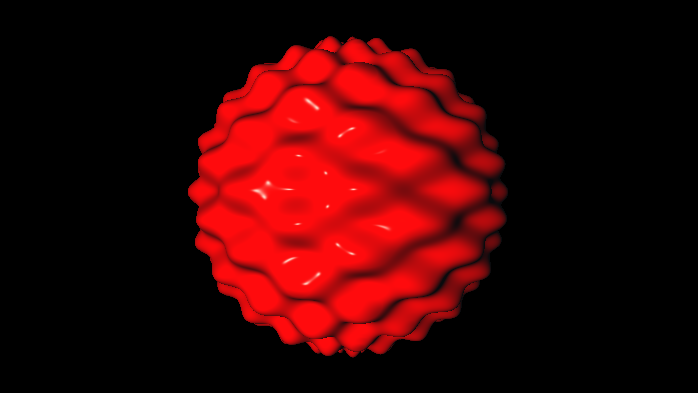
\includegraphics[width=.6\linewidth]{imagens/sdf-distortion/sin-cos-distortion.png}
  \captionof{figure}{Distortion on Sphere from Code 7}
  \label{fig:sin-cos-distortion}
\end{figure}

In Code 7, the Sphere Distance is distorted according to the trigonometric functions applied on its polar and azimutal angle. The result is shown in Figure \ref{fig:sin-cos-distortion}.
\chapter{Clouds}\label{chp:LABEL_CHP_4}

One of the main applications of Ray Marching is in the rendering of realistic smoke, clouds, which are called volumetric objects. Clouds are mostly made of two main high-albedo types of particles, if not considering dirt or other minimal particles: air and water/ice. \cite{:REF_IN_1}
Since clouds are not solid, when light hits them, some rays bounce, but some go through the object. Not only that, the water particles are anisotropic\cite{:REF_IN_1}, which means that light tends to bounce differently depending on the direction from which it hits the cloud. All in all, there is a lot to adapt from the original Ray Marching concocted. 

\section{Volumetric Rendering}

Firstly, to render gaseous materials, instead of avoiding going into surfaces, Ray Marching needs to go through the clouds. For that, the SDF now represents density instead of "distance to surface". For the sake of clarity, the SDFs are inversed so that the distance to a point is as follows. 

\begin{itemize}
    \item Outside of the primitive, yields a negative density, or no density.
    \item Inside of the primitive, yields a positive density, and the further the point is from bounds, the higher the density is.
\end{itemize}

Secondly, to consistently sample the density along the cloud, a constant step size is better suited - instead of querying the scene's distance for the next marching step, each step will perform a constant size.

\begin{algorithm}[H]
\caption{MarchRay}
\label{alg:marchray}
\begin{algorithmic}[1]
\Procedure{MarchRay}{RayOrigin, RayDirection, Scene}
    \State $ \mathbf{MarchDistance} \gets \text{0} $
    \State $ \mathbf{Hit} \gets \text{NULL\_HIT} $
    \State $ \mathbf{IsHit} \gets \text{false} $
    \For {$step \gets 0$ to $\text{MAX\_MARCH\_STEPS} - 1$}
        \State $\mathbf{MarchPos} \gets  RayOrigin+ (MarchDistance * RayDirection) $
        \State $\mathbf{Hit} \gets \Call{GetDistance}{MarchPos, scene}$
        \If{$\text{Hit.distance} < \text{SURFACE\_DISTANCE}$}
            \State $ \mathbf{IsHit} \gets \text{true} $
            \State $ break $
        \EndIf
        \If{$\text{MarchDistance} > \text{MAX\_MARCH\_DISTANCE}$}
            \State $ break $
        \EndIf
    \EndFor
    \State \Return $\mathbf{Hit}$
\EndProcedure
\end{algorithmic}
\end{algorithm}


\section{Noise}



\section{Volumetric Shading}

% \begin{figure}[ht]
%     \centering
%     \fbox{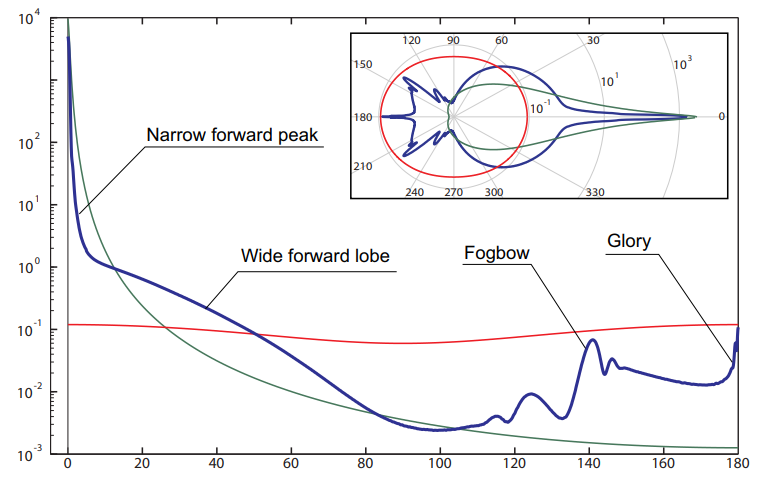
\includegraphics[width=9.5cm]{imagens/phase_functions.png}}
%     \caption{Log plots (inset: polar log plots) of commonly used phase functions. Red: Rayleigh. Green: Henyey-Greenstein with g = .99. Blue: Mie. Extracted from \cite{:REF_IN_2}}.
%     \label{fig:square_sdf}
% \end{figure}
\chapter{Conclusion and Future Works}\label{chp:LABEL_CHP_5}

% Mencionar outros metodos de obter formas complexas como:
% GRIDS: https://renderdiagrams.org/2017/12/28/signed-distance-fields/
% https://steamcdn-a.akamaihd.net/apps/valve/2007/SIGGRAPH2007_AlphaTestedMagnification.pdf
% NEURAL NETWORKS: 
\pagebreak

%%%%%%%%%%%%%%%%%%%%%%%%%%%%%%%%%%%%%%%%%%%%%%%%%%%%%%%%%%%%
% B I B L I O G R A F I A
%%%%%%%%%%%%%%%%%%%%%%%%%%%%%%%%%%%%%%%%%%%%%%%%%%%%%%%%%%%%
% Retirar esta parte se o trabalho não tiver bibliografia
\makebibspage{abnt}{elementos-postextuais/referencias}


%%%%%%%%%%%%%%%%%%%%%%%%%%%%%%%%%%%%%%%%%%%%%%%%%%%%%%%%%%%%
% G L O S S A R I O (opcional)
%%%%%%%%%%%%%%%%%%%%%%%%%%%%%%%%%%%%%%%%%%%%%%%%%%%%%%%%%%%%
\makeglossarypage{\item [Palavra] Significado da palavra

\item [Palavra 2] Significado da palavra 2

}

%%%%%%%%%%%%%%%%%%%%%%%%%%%%%%%%%%%%%%%%%%%%%%%%%%%%%%%%%%%%
% A N E X O (opcional)
%%%%%%%%%%%%%%%%%%%%%%%%%%%%%%%%%%%%%%%%%%%%%%%%%%%%%%%%%%%%
\annex
\annexchapter{A}{Lorem ipsum dolor sit amet}

Lorem ipsum dolor sit amet, consectetur adipiscing elit. Donec lacus nisl, ultricies vitae semper eu, scelerisque nec enim. Curabitur posuere tortor orci, at porta leo laoreet et. Quisque ut congue dolor. Maecenas vel sagittis diam. Praesent fermentum eleifend mi, sit amet vehicula leo pellentesque quis. Curabitur mattis luctus pulvinar. Proin auctor est nec nulla pellentesque commodo. Donec nec justo eu magna aliquet eleifend. Curabitur tristique tortor id sem dignissim, a iaculis metus interdum. Phasellus bibendum velit sit amet interdum semper. Nam vestibulum dui quis nisi consectetur, id vehicula dolor faucibus.
\annexchapter{B}{Lorem ipsum dolor sit amet}

Lorem ipsum dolor sit amet, consectetur adipiscing elit. Donec lacus nisl, ultricies vitae semper eu, scelerisque nec enim. Curabitur posuere tortor orci, at porta leo laoreet et. Quisque ut congue dolor. Maecenas vel sagittis diam. Praesent fermentum eleifend mi, sit amet vehicula leo pellentesque quis. Curabitur mattis luctus pulvinar. Proin auctor est nec nulla pellentesque commodo. Donec nec justo eu magna aliquet eleifend. Curabitur tristique tortor id sem dignissim, a iaculis metus interdum. Phasellus bibendum velit sit amet interdum semper. Nam vestibulum dui quis nisi consectetur, id vehicula dolor faucibus.

\end{document}